\documentclass[12pt]{article}
\usepackage{graphicx}
\usepackage{geometry}
\usepackage{xcolor}
\usepackage{tikz}
\usepackage{hyperref}

\hypersetup{colorlinks=true,linkcolor=black,urlcolor=black}

% Shape for flowchart
\tikzstyle{startstop} = [rectangle, rounded corners, minimum width=3cm, minimum height=1cm, text centered, draw=black, fill=red!30]
\tikzstyle{decision} = [rectangle, minimum width=3cm, minimum height=1cm, text centered, draw=black, fill=green!30]
\tikzstyle{process} = [rectangle, minimum width=3cm, minimum height=1cm, text centered, text width=3cm, draw=black, fill=orange!30]
\tikzstyle{arrow} = [thick,->,>=stealth]

% Page Margins
\geometry{a4paper, margin=1in}

\begin{document}

\begin{titlepage}
    \centering
    % Image and Title
    \includegraphics[width=0.5\textwidth]{assets/logo.png}\par\vspace{1cm}
    % Title
    \Huge\textbf{Rebackk Whitepaper} \\
    % Subtitle
    \Large\textbf{Repel, Regain, Rebackk} \\[1cm]
    % Author and Date
    \large
    \textbf{Author:}  Rebackk Team \\
    \textbf{Date:} \today 
    % Whitespace
    \vfill
    % Product name and website
    \textbf{Rebackk} \\
    \textbf{www.rebackk.xyz}
\end{titlepage}

% Table of Contents
\tableofcontents
\newpage

\section{Introduction}

\subsection{Overview}

This whitepaper introduces Rebackk, a revolutionary data protection solution designed to empower businesses of all sizes in today's ever-evolving digital landscape. By leveraging the power of blockchain technology, Rebackk provides unparalleled security, automated backups, and seamless data recovery, ensuring your business continuity and peace of mind.

\subsection{The Problem}

In today's data-driven world, businesses face a constant threat: data loss. From cyberattacks like ransomware to accidental deletion and hardware failures, even a minor incident can lead to devastating consequences. Data breaches are on the rise, costing companies millions of dollars due to compromised information. Accidental deletion wipes out critical files, and hardware malfunctions or natural disasters can result in permanent data loss. These events not only cause financial harm but also damage a company's reputation and lead to legal repercussions.

\subsection{The Rebackk Solution}

Rebackk offers a groundbreaking solution to these challenges. Our innovative platform utilizes blockchain technology, a decentralized and tamper-proof ledger, to ensure the security and immutability of your data backups. This means your data is always protected, even in the event of a cyberattack or hardware failure. Rebackk automates the entire backup process, eliminating the risk of human error and ensuring your data is always up-to-date. Encrypted storage provides an additional layer of security, and Rebackk's intuitive interface allows for effortless data recovery when needed.

\subsection{Benefits of Rebackk}

With Rebackk, businesses gain peace of mind knowing their data is safe and readily accessible. Rebackk offers several key benefits:

\begin{enumerate}
    \item \textbf{Unparalleled Security}: Blockchain technology ensures the immutability and security of your backups.
    \item \textbf{Automated Backups}: Eliminate the risk of human error with automated backup processes.
    \item \textbf{Effortless Recovery}: Recover lost data quickly and easily with Rebackk's intuitive interface.
    \item \textbf{Disaster Recovery}: Rebackk helps businesses recover from unexpected events and ensures business continuity.
    \item \textbf{Regulatory Compliance}: Secure storage and automated backups facilitate compliance with data protection regulations.
\end{enumerate}

By choosing Rebackk, businesses can focus on their core operations while we take care of their data security needs.

\newpage

% Problem Statement
% Problem Statement Section Should Have:
%  - Clearly define the cybersecurity issue or challenge that organizations face.
% - Discuss the implications and risks associated with this problem.
% - Provide statistics or examples to support your claims.
\section{Problem Statement}

\subsection{Definition}

Data loss is a constant threat for organizations of all sizes. It can occur due to a variety of reasons, including:

\begin{enumerate}
    \item \textbf{Cyberattacks:} Ransomware attacks, phishing scams, and malware infections can all lead to data breaches and data loss.
    \item \textbf{Accidental Deletion:} Human error is a surprisingly common cause of data loss. Employees may accidentally delete critical files or folders.
    \item \textbf{Hardware Failures:} Hardware malfunctions, such as hard drive failures or power outages, can result in permanent data loss.
    \item \textbf{Natural Disasters:} Fires, floods, and other natural disasters can damage hardware and destroy data.
\end{enumerate}

\subsection{Implications}

The implications of data loss can be devastating for businesses. Here are some of the key risks:

\begin{enumerate}
    \item \textbf{Financial Loss:} Data loss can lead to significant financial losses. Companies may need to pay for data recovery services, replace lost equipment, and compensate clients for compromised information.
    \item \textbf{Reputational Damage:} A data breach can seriously damage a company's reputation. Customers may lose trust in a company that cannot protect their data.
    \item \textbf{Legal Repercussions:} Depending on the type of data lost, companies may face legal repercussions for non-compliance with data protection regulations.
    \item \textbf{Operational Disruption:} Data loss can disrupt a company's operations, leading to lost productivity and downtime.
\end{enumerate}

\subsection{Statistics}

The severity of data loss is underscored by statistics:

\begin{enumerate}
    \item \textbf{Cyberattacks:} According to the 2021 Cost of a Data Breach Report by IBM, the average cost of a data breach is \$4.24 million.
    \item \textbf{Human Error:} A study by the IT Policy Compliance Group found that 80\% of data loss is due to human error.
    \item \textbf{Hardware Failures:} The Ponemon Institute's 2021 Data Risk in the Third-Party Ecosystem report found that 40\% of organizations experienced a data breach due to hardware failure.
    \item \textbf{Loss of trust} A survey by Ping Identity found that 78\% of consumers would stop engaging with a brand online after a data breach.
    \item \textbf{Legal Repercussions:} The General Data Protection Regulation (GDPR) imposes fines of up to 4\% of a company's annual global turnover for non-compliance.
    \item \textbf{Operational Disruption:} A study by Gartner found that the average cost of IT downtime is \$5,600 per minute.
    \item \textbf{Small Businesses:} According to the National Cyber Security Alliance, 60\% of small businesses go out of business within six months of a cyberattack.
    \item \textbf{Data Recovery:} The Data Recovery Institute found that 96\% of companies with a reliable backup and recovery plan were able to survive ransomware attacks.
    \item \textbf{Data Protection:} A survey by the Ponemon Institute found that 68\% of organizations do not have a data protection strategy in place.
    \item \textbf{Business Continuity:} The Disaster Recovery Preparedness Council found that 3 out of 4 companies worldwide are not prepared for a disaster.
\end{enumerate}

These statistics highlight the prevalence and serious consequences of data loss for businesses.

\section{Solution Overview}

\subsection{How Rebackk Works}

Rebackk offers a revolutionary solution to the ever-present threat of data loss. Our innovative platform leverages a custom zkRollup blockchain, built on our in-house blockchain infrastructure, to provide unparalleled security, automated backups, and seamless data recovery. Here's how Rebackk works:

\begin{enumerate}
    \item \textbf{Automated Backups}: Rebackk automates the entire backup process, eliminating the risk of human error. You can schedule regular backups to ensure your data is always up-to-date.
    \item \textbf{Secure Storage with zkRollup Technology}: Rebackk utilizes a custom zkRollup blockchain built on our secure in-house blockchain infrastructure. This zkRollup technology offers several advantages:
        * **Enhanced Scalability:** ZkRollups can process a high volume of transactions efficiently, ensuring smooth operation even as your data storage needs grow.
        * **Unparalleled Security:** ZkRollups inherit the security benefits of our underlying blockchain, while keeping transaction data confidential. Only cryptographic proofs of validity are stored on the main chain, minimizing the attack surface.
    \item \textbf{Effortless Recovery}: With Rebackk, recovering lost data is a breeze.  Our intuitive interface allows you to easily identify and restore specific files or entire folders in just a few clicks.
\end{enumerate}

\subsection{Key Features}

Rebackk empowers businesses with a comprehensive suite of features designed to simplify data protection:

\begin{enumerate}
    \item \textcolor{black}{\bfseries}Centralized Management\textcolor{black}{\normalfont}: Manage all your backups from a single, user-friendly dashboard.
    \item \textcolor{black}{\bfseries}Granular Access Control\textcolor{black}{\normalfont}: Set access permissions for different users and teams to ensure data security.
    \item \textcolor{black}{\bfseries}Version Control\textcolor{black}{\normalfont}: Rebackk maintains a history of your backups, allowing you to restore previous versions of files if needed.
    \item \textcolor{black}{\bfseries}Compliance Management\textcolor{black}{\normalfont}: Rebackk helps businesses meet various data protection regulations with its secure storage and automated processes.
    \item \textcolor{black}{\bfseries}Scalability\textcolor{black}{\normalfont}: Rebackk seamlessly scales to accommodate your growing data storage needs, thanks to the efficient zkRollup technology.
\end{enumerate}

\subsection{Technology Behind Rebackk}

The cornerstone of Rebackk's security lies in our custom zkRollup blockchain, built on top of our in-house blockchain infrastructure. ZkRollups offer significant advantages for data storage:
\begin{enumerate}
    \item \textbf{Scalability}: ZkRollups can process a high volume of transactions efficiently, ensuring smooth operation even as your data storage needs grow.
    \item \textbf{Security}: ZkRollups inherit the security benefits of our underlying blockchain, while keeping transaction data confidential. Only cryptographic proofs of validity are stored on the main chain, minimizing the attack surface.
    \item \textbf{Efficiency}: ZkRollups provide a cost-effective solution for data storage, reducing the overhead associated with traditional blockchain transactions.
    \item \textbf{Privacy}: ZkRollups ensure the privacy of your data by keeping transaction details confidential, while still providing cryptographic proofs of validity.
\end{enumerate}

In addition to zkRollups, Rebackk utilizes various security protocols to further safeguard your data. These include encryption at rest and in transit, access controls, and regular security audits.

\subsubsection{Custom Rollup and Blockchain Solutions (Optional)}

Rebackk's expertise extends beyond its core data protection platform. We offer a unique service:

\begin{enumerate}
    \item \textbf{Customizable Blockchain and Rollup Development}: Our team can develop custom blockchain and zkRollup solutions tailored to your specific needs. This allows you to leverage the power of blockchain technology for various applications beyond data backup.
\end{enumerate}
\newpage


% Technical Details
% Technical Details Section Should Have:
% - Provide deeper technical insights into how our product works.
% - Discuss any algorithms, protocols, or technologies used.
% - Include architecture diagrams or flowcharts if applicable.
\section{Technical Details}

This section delves deeper into the technical aspects of Rebackk, offering insights into the algorithms, protocols, and technologies that power our secure and efficient data protection platform.

\subsection{Algorithms}

Rebackk leverages a combination of algorithms to ensure optimal performance and data integrity:

\begin{enumerate}
    \item \textbf{Data Deduplication}: Rebackk utilizes efficient data deduplication algorithms to minimize storage requirements. These algorithms identify and store only unique data chunks, reducing redundancy and optimizing storage space.
    \item \textbf{Incremental Backups}: Rebackk employs intelligent algorithms to perform incremental backups. These algorithms identify and back up only the data that has changed since the last backup, minimizing bandwidth usage and backup times.
\end{enumerate}

\subsection{Protocols}
\begin{enumerate}
    \item \textbf{Zero-knowledge proofs (ZKPs)}: ZKPs are a cornerstone of zkRollup technology. They allow Rebackk to verify the validity of transactions without revealing the actual data content. This ensures data confidentiality while maintaining blockchain security.
    \item \textbf{Secure Multi-party Computation (SMPC)}: Rebackk may utilize SMPC protocols in certain functionalities to enable secure computations on encrypted data without decryption. This further enhances data privacy while facilitating specific operations.
\end{enumerate}

\subsection{Architecture}
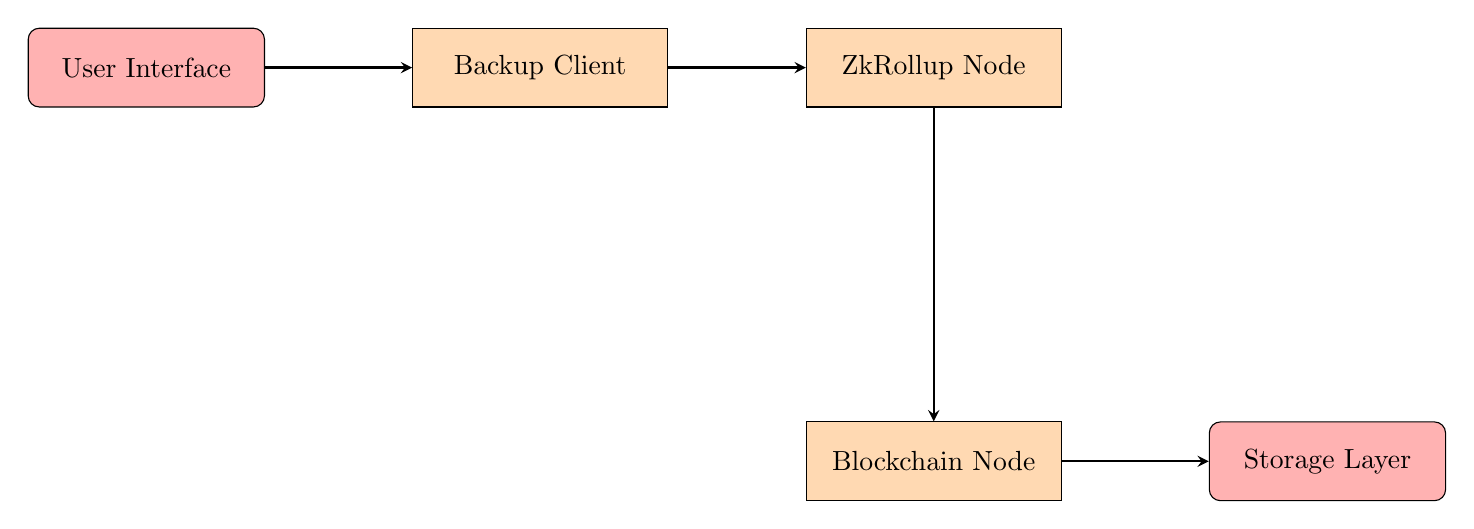
\begin{tikzpicture}[node distance=5cm, align=center]

    % Nodes
    \node (ui) [startstop] {User Interface};
    \node (bc) [process, right of=ui] {Backup Client};
    \node (zk) [process, right of=bc] {ZkRollup Node};
    \node (bn) [process, below of=zk] {Blockchain Node};
    \node (sl) [startstop, right of=bn] {Storage Layer};
    
    % Arrows
    \draw [arrow] (ui) -- (bc);
    \draw [arrow] (bc) -- (zk);
    \draw [arrow] (zk) -- (bn);
    \draw [arrow] (bn) -- (sl);

\end{tikzpicture}
\label{fig:architecture}

\subsection{Flowcharts}
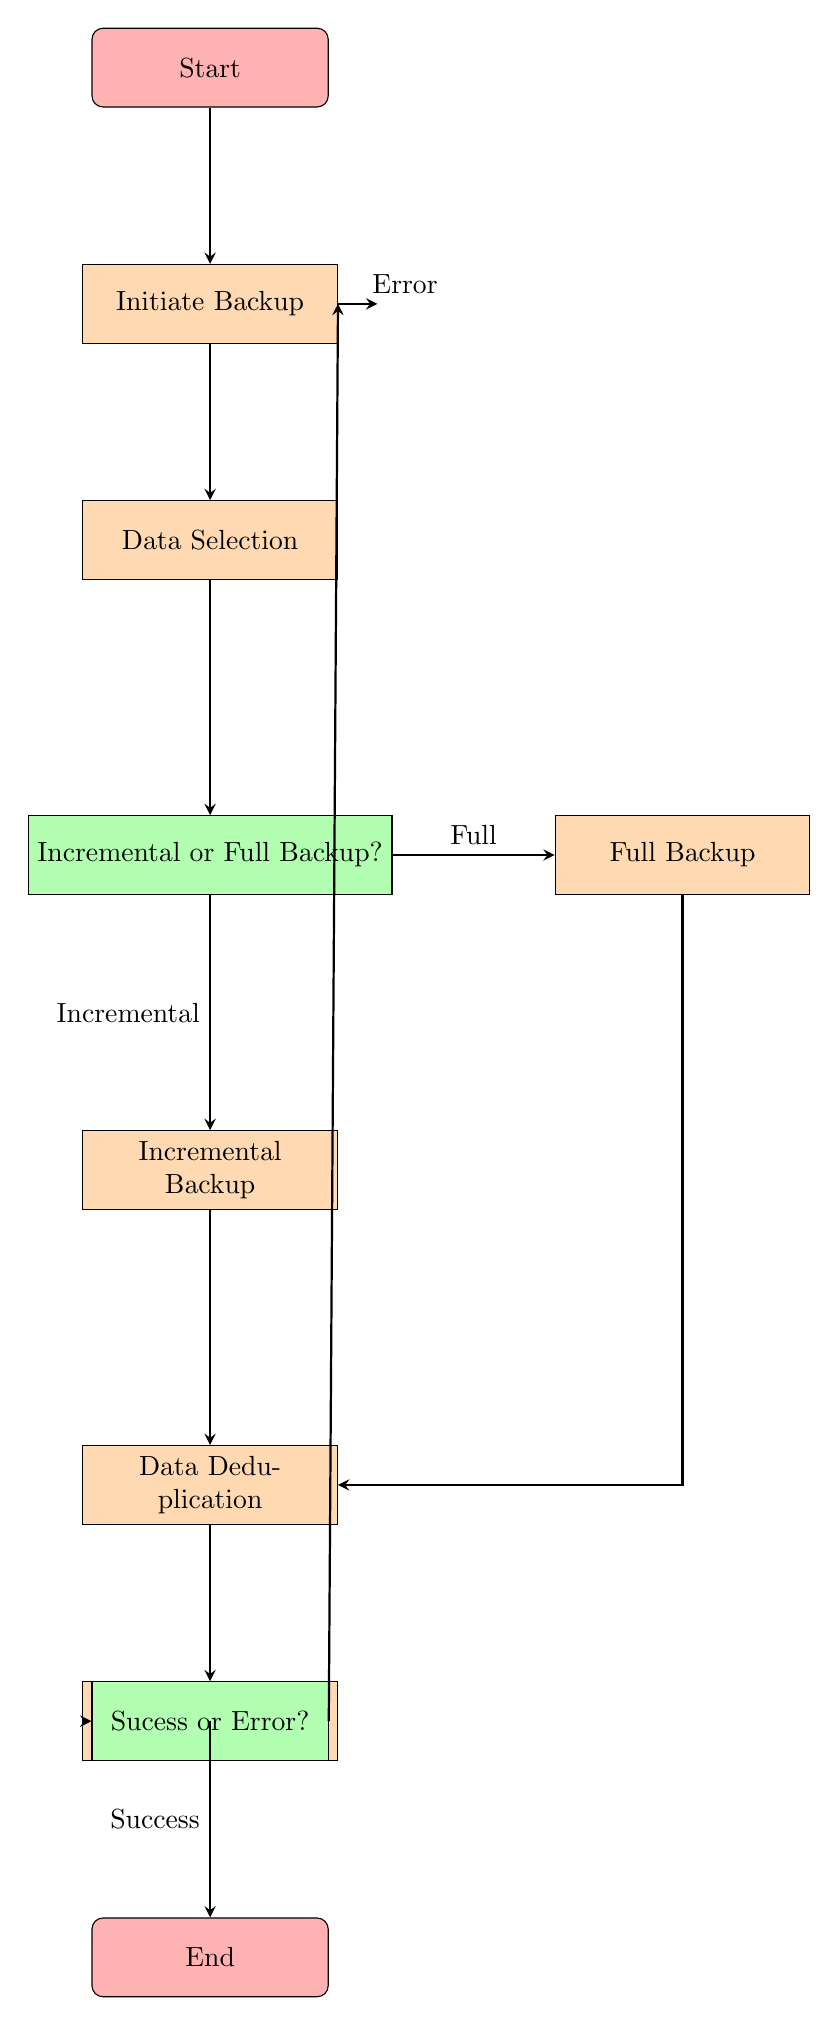
\begin{tikzpicture}[node distance=3cm]
    % Flowchart nodes
    \node (start) [startstop] {Start};
    \node (backup) [process, below of=start] {Initiate Backup};
    \node (dedup) [process, below of=backup] {Data Selection};
    \node (incorfull) [decision, below of=dedup, yshift=-1cm] {Incremental or Full Backup?};
    \node (inc) [process, below of=incorfull, yshift=-1cm] {Incremental Backup};
    \node (full) [process, right of=incorfull, xshift=3cm] {Full Backup};
    \node (encrypt) [process, below of=inc, yshift=-1cm] {Data Deduplication};
    \node (store) [process, below of=encrypt] {Data Transfer};
    \node (sucorerror) [decision, below of=encrypt] {Sucess or Error?};
    \node (end) [startstop, below of=sucorerror] {End};

    % Arrows
    \draw [arrow] (start) -- (backup);
    \draw [arrow] (backup) -- (dedup);
    \draw [arrow] (dedup) -- (incorfull);
    \draw [arrow] (incorfull) -- node[anchor=east] {Incremental} (inc);
    \draw [arrow] (incorfull) -- node[anchor=south] {Full} (full);
    \draw [arrow] (full) |- (encrypt);
    \draw [arrow] (inc) -- (encrypt);
    \draw [arrow] (encrypt) -- (store);
    \draw [arrow] (store) -- (sucorerror.west);
    \draw [arrow] (sucorerror.center) -- node[anchor=east] {Success} (end);
    \draw [arrow] (sucorerror.east) -- (backup.east);
    \draw [arrow] (backup.east) -- ++(0.5,0) node[anchor=south , xshift=10] {Error};
\end{tikzpicture}
\label{fig:flowchart}

\subsection{Technologies}

Beyond the core functionalities mentioned above, Rebackk incorporates various additional technologies:

\begin{enumerate}
    \item \textbf{Encryption}: Rebackk utilizes robust encryption algorithms to protect data at rest and in transit. This ensures data confidentiality even in the event of a security breach.
    \item \textbf{Access Control}: Granular access controls allow you to define user permissions and restrict access to sensitive data.
    \item \textbf{Auditing and Logging}: Rebackk maintains comprehensive audit logs to track user activity and data access attempts. This facilitates security monitoring and compliance efforts.
\end{enumerate}

By combining these algorithms, protocols, and technologies, Rebackk delivers a secure, efficient, and auditable data protection solution.

% Use Cases:
% Use Cases Section Should Have:
% - Present practical scenarios or examples where our product can be applied.
% - Describe specific industries or sectors that can benefit from our solution.
\section{Use Cases}
Rebackk empowers businesses of all sizes to safeguard their valuable data with a comprehensive data protection solution. This section delves into practical scenarios where Rebackk proves invaluable, explores industries that can particularly benefit from its features.

\subsection{Scenarios}
Rebackk addresses a wide range of data protection challenges faced by businesses today. Here are some common scenarios where Rebackk shines:

\begin{itemize}
    \item \textbf{Accidental Data Deletion}: Human error is inevitable. Rebackk's automated backups ensure critical data is always protected. With its intuitive interface, users can easily recover lost files or entire folders in just a few clicks, minimizing downtime and data loss.
    \item \textbf{Hardware Failure}: Hardware malfunctions can lead to data loss. Rebackk's secure, off-site storage on the zkRollup blockchain ensures your data remains safe and readily available for recovery, even in the event of a server crash.
    \item \textbf{Ransomware Attcks}:  Malicious cyberattacks pose a significant threat. Rebackk's immutable backups, stored on the tamper-proof blockchain, provide a clean, uninfected copy for data restoration. This minimizes the impact of ransomware attacks and helps businesses recover quickly.
    \item \textbf{Regulatory Compliance}: Businesses in healthcare, finance, or other regulated industries can leverage Rebackk to meet data retention and security compliance requirements. Rebackk's secure storage and comprehensive audit trails simplify the compliance process.
\end{itemize}

By providing automated backups, effortless recovery, and secure storage, Rebackk empowers businesses to face these challenges with confidence.

\subsection{Industries}
Rebackk's robust data protection solution caters to the diverse needs of various industries. Here are some sectors that can significantly benefit from Rebackk's capabilities:

\begin{itemize}
    \item \textbf{Healthcare}: Healthcare organizations handle sensitive patient data that must be protected at all costs. Rebackk's secure storage and automated backups ensure compliance with HIPAA regulations and safeguard patient information.
    \item \textbf{Finance}: Financial institutions deal with vast amounts of confidential data, making them prime targets for cyberattacks. Rebackk's immutable backups and secure storage help financial organizations protect their data and maintain business continuity.
    \item \textbf{Legal}: Law firms store critical case files and client information that must be safeguarded. Rebackk's granular access controls and audit logs ensure data security and compliance with legal industry regulations.
    \item \textbf{E-commerce}: Online retailers rely on customer data for marketing and sales. Rebackk's automated backups and efficient recovery mechanisms help e-commerce businesses protect customer information and maintain operational continuity.
    \item \textbf{Education}: Educational institutions store vast amounts of student and faculty data. Rebackk's secure storage and version control features help schools and universities protect their data and ensure seamless operations.
\end{itemize}

% Key Features and Benefits
% Key Features and Benefits Section Should Have:
% - List and elaborate on the unique features of our product.
% - Explain the advantages and benefits that customers will experience.
% - How We Plan To Differentiate our product from competitors in terms of features and benefits.
\section{Key Features and Benefits}
Rebackk empowers businesses with a comprehensive data protection solution that safeguards valuable information and ensures its accessibility. This section explores the unique features of Rebackk, the resulting advantages it offers, and how it stands out from the competition.

\subsection{Unique Features}
Rebackk leverages cutting-edge technology to provide a robust and user-friendly data protection solution. Here are some key features that distinguish Rebackk:

\begin{itemize}
    \item \textbf{Automated Backups}: Rebackk automates the backup process, eliminating the risk of human error and ensuring your data is always up-to-date.
    \item \textbf{Secure Storage with zkRollup Technology}: Rebackk utilizes a custom zkRollup blockchain to provide secure and tamper-proof storage for your backups.
    \item \textbf{Effortless Recovery}: With Rebackk's intuitive interface, recovering lost data is quick and easy, minimizing downtime and data loss.
    \item \textbf{Granular Access Control}: Rebackk allows you to set access permissions for different users and teams, ensuring data security and compliance.
    \item \textbf{Version Control}: Rebackk maintains a history of your backups, enabling you to restore previous versions of files if needed.
    \item \textbf{Compliance Management}: Rebackk helps businesses meet various data protection regulations with its secure storage and automated processes.
    \item \textbf{Scalability}: Rebackk seamlessly scales to accommodate your growing data storage needs, thanks to the efficient zkRollup technology.
    \item \textbf{Efficient Deduplication}: Rebackk employs data deduplication algorithms to minimize storage requirements and optimize backup efficiency.
    \item \textbf{Comprehensive Audit Logging}: Rebackk maintains detailed audit logs to track user activity and data access attempts, facilitating security monitoring and compliance efforts.
\end{itemize}

These unique features provide a solid foundation for Rebackk's comprehensive data protection solution.

\subsection{Advantages}
By leveraging its unique features, Rebackk offers several advantages to its users:

\begin{itemize}
    \item \textbf{Enhanced Security}: Rebackk's secure storage on the zkRollup blockchain ensures the immutability and confidentiality of your backups, protecting your data from cyber threats.
    \item \textbf{Automated Processes}: Rebackk's automated backups and efficient recovery mechanisms minimize the risk of data loss due to human error or hardware failures.
    \item \textbf{Compliance Assistance}: Rebackk helps businesses meet data protection regulations by providing secure storage, granular access controls, and comprehensive audit trails.
    \item \textbf{Scalability}: Rebackk seamlessly scales to accommodate your growing data storage needs, ensuring your data protection solution grows with your business.
    \item \textbf{Efficient Data Management}: Rebackk's data deduplication algorithms optimize storage space and backup efficiency, reducing costs and improving performance.
    \item \textbf{User-Friendly Interface}: Rebackk's intuitive interface makes it easy to manage backups, recover lost data, and monitor user activity, enhancing user experience and productivity.
    \item \textbf{Business Continuity}: Rebackk helps businesses recover quickly from data loss incidents, ensuring operational continuity and minimizing downtime.
    \item \textbf{Cost-Effective Solution}: Rebackk's efficient data management and automated processes reduce the overhead associated with data protection, providing a cost-effective solution for businesses of all sizes.
    \item \textbf{Customizable Solutions}: Rebackk offers customizable blockchain and zkRollup solutions tailored to your specific needs, allowing you to leverage the power of blockchain technology for various applications.
\end{itemize}

These advantages translate into tangible benefits for businesses of all sizes.

\subsection{Differentiation}
The competitive landscape for data protection solutions is crowded. However, Rebackk differentiates itself through several key aspects:

\begin{itemize}
    \item \textbf{Blockchain Technology}: Rebackk's use of zkRollup blockchain technology provides unparalleled security and immutability for your backups, setting it apart from traditional data protection solutions.
    \item \textbf{Automated Backups}: Rebackk's automated backup processes eliminate the risk of human error and ensure your data is always protected and up-to-date, offering a seamless and efficient solution.
    \item \textbf{Effortless Recovery}: Rebackk's intuitive interface makes data recovery quick and easy, minimizing downtime and data loss, and enhancing user experience.
    \item \textbf{Compliance Management}: Rebackk helps businesses meet data protection regulations with its secure storage, granular access controls, and comprehensive audit trails, simplifying compliance efforts.
    \item \textbf{Scalability}: Rebackk seamlessly scales to accommodate your growing data storage needs, ensuring your data protection solution grows with your business, providing long-term value.
\end{itemize}

By combining these differentiating factors, Rebackk establishes itself as a compelling choice for businesses seeking a secure, user-friendly, and cost-effective data protection solution.

% Implementation
% Implementation Section Should Have:
% - Outline how easy it is to implement our product.
% - Discuss integration with existing systems or workflows.
\section{Implementation}
Rebackk is designed for seamless integration into your existing workflows, minimizing disruption and ensuring a smooth onboarding experience. This section explores the ease of implementation and Rebackk's integration capabilities.

\subsection{Ease of Implementation}
Rebackk prioritizes user experience with a straightforward and intuitive setup process. Here's what makes implementing Rebackk simple:

\begin{enumerate}
    \item \textbf{User-Friendly Interface}: Rebackk's user-friendly interface guides you through the setup process, making it easy to configure your backup settings and schedule automated backups.
    \item \textbf{Step-by-Step Instructions}: Rebackk provides clear, step-by-step instructions to help you get started quickly and easily, ensuring a smooth onboarding experience.
    \item \textbf{Customizable Settings}: Rebackk allows you to customize backup settings to suit your specific needs, ensuring that the solution aligns with your data protection requirements.
    \item \textbf{Technical Support}: Rebackk offers technical support to assist you with any questions or issues during the implementation process, providing peace of mind and ensuring a successful deployment.
    \item \textbf{Training Resources}: Rebackk provides training resources, documentation, and tutorials to help you make the most of the platform and optimize your data protection strategy.
    \item \textbf{Scalable Architecture}: Rebackk's scalable architecture allows you to expand your data storage needs seamlessly as your business grows, ensuring long-term value and flexibility.
    \item \textbf{Customizable Solutions}: Rebackk offers customizable blockchain and zkRollup solutions tailored to your specific needs, allowing you to leverage the power of blockchain technology for various applications.
    \item \textbf{Integration with Existing Systems}: Rebackk integrates seamlessly with your existing systems and workflows, minimizing disruption and ensuring a smooth transition to the new data protection solution.
    \item \textbf{Comprehensive Support}: Rebackk provides comprehensive support throughout the implementation process, from initial setup to ongoing maintenance, ensuring that your data protection needs are met effectively.
\end{enumerate}

By prioritizing user experience with a cloud-based solution, minimal configuration, and comprehensive support, Rebackk simplifies the implementation process and allows you to focus on your core business activities.

\subsection{Integration}
Rebackk understands the importance of seamlessly integrating with existing systems to minimize disruption and maximize efficiency. Here's how Rebackk facilitates integration:
\begin{itemize}
    \item \textbf{API Integration}: Rebackk offers API integration capabilities, allowing you to connect Rebackk with your existing systems and workflows, enabling data exchange and automation.
    \item \textbf{Customizable Solutions}: Rebackk provides customizable blockchain and zkRollup solutions tailored to your specific needs, ensuring seamless integration with your existing infrastructure.
    \item \textbf{Pre-built Connectors}: Rebackk offers pre-built connectors for popular platforms and applications, simplifying the integration process and accelerating time to value.
    \item \textbf{Data Migration Support}: Rebackk provides data migration support to help you transfer your existing data to the Rebackk platform, ensuring a smooth transition and minimal downtime.
\end{itemize}

By offering API access, pre-built connectors, and customization options, Rebackk empowers you to integrate data protection seamlessly into your existing workflows, maximizing efficiency and minimizing disruption.

% Security and Compliance
% Security and Compliance Section Should Have:
% - Detail the security measures implemented in our product.
% - Address compliance with industry standards or regulations (e.g., GDPR, HIPAA).
% - Explain how our product protects data and ensures privacy.
\section{Security and Compliance}
Rebackk prioritizes the security and integrity of your data. This section delves into the robust security measures implemented within Rebackk, its compliance with industry standards, and how it safeguards your data privacy.

\subsection{Security Measures}
Rebackk employs a multi-layered security approach to ensure the complete protection of your data:

\begin{itemize}
    \item \textbf{Encryption at Rest and in Transit}: Rebackk encrypts your data both at rest and in transit, ensuring that your backups are secure and protected from unauthorized access.
    \item \textbf{Access Controls}: Rebackk provides granular access controls, allowing you to define user permissions and restrict access to sensitive data, enhancing data security and privacy.
    \item \textbf{Audit Logging}: Rebackk maintains comprehensive audit logs to track user activity and data access attempts, facilitating security monitoring and compliance efforts.
    \item \textbf{Secure Storage on zkRollup Blockchain}: Rebackk stores your backups on a custom zkRollup blockchain, providing tamper-proof and immutable storage for your data, ensuring its security and integrity.
    \item \textbf{Zero-knowledge Proofs (ZKPs)}: Rebackk utilizes ZKPs to verify the validity of transactions without revealing the actual data content, ensuring data confidentiality while maintaining blockchain security.
    \item \textbf{Secure Multi-party Computation (SMPC)}: Rebackk may utilize SMPC protocols in certain functionalities to enable secure computations on encrypted data without decryption, further enhancing data privacy and security.
    \item \textbf{Regular Security Audits}: Rebackk undergoes regular security audits to identify and address potential vulnerabilities, ensuring that your data is protected from emerging threats.
    \item \textbf{Data Deduplication}: Rebackk employs data deduplication algorithms to minimize storage requirements and optimize backup efficiency, reducing costs and improving performance.
    \item \textbf{Efficient Data Management}: Rebackk's data deduplication algorithms optimize storage space and backup efficiency, reducing costs and improving performance.
\end{itemize}
By implementing these comprehensive security measures, Rebackk offers a secure environment for your valuable data.

\subsection{Compliance}
Rebackk understands the importance of adhering to industry regulations and data privacy laws. Our solution is designed to facilitate compliance with various standards, including:

\begin{itemize}
    \item \textbf{General Data Protection Regulation (GDPR)}: Rebackk helps businesses comply with the GDPR by providing secure storage, granular access controls, and comprehensive audit trails.
    \item \textbf{Health Insurance Portability and Accountability Act (HIPAA)}: Rebackk ensures compliance with HIPAA regulations by safeguarding patient data with encryption, access controls, and audit logging.
    \item \textbf{Payment Card Industry Data Security Standard (PCI DSS)}: Rebackk helps businesses meet PCI DSS requirements by protecting payment card data with secure storage and access controls.
    \item \textbf{Sarbanes-Oxley Act (SOX)}: Rebackk facilitates compliance with SOX regulations by providing secure storage, audit trails, and access controls for financial data.
    \item \textbf{California Consumer Privacy Act (CCPA)}: Rebackk ensures compliance with the CCPA by protecting consumer data with encryption, access controls, and audit logging.
    \item \textbf{ISO/IEC 27001}: Rebackk aligns with ISO/IEC 27001 standards by implementing robust security measures, encryption, access controls, and audit logging to protect data.
\end{itemize}

By adhering to these regulations, Rebackk empowers you to manage your data with confidence, knowing it is protected and handled according to industry best practices.

\subsection{Data Protection}
Data privacy is a core principle at Rebackk. Here's how we ensure the protection of your data:

\begin{itemize}
    \item \textbf{Encryption}: Rebackk encrypts your data both at rest and in transit, ensuring that your backups are secure and protected from unauthorized access.
    \item \textbf{Access Controls}: Rebackk provides granular access controls, allowing you to define user permissions and restrict access to sensitive data, enhancing data security and privacy.
    \item \textbf{Zero-knowledge Proofs (ZKPs)}: Rebackk utilizes ZKPs to verify the validity of transactions without revealing the actual data content, ensuring data confidentiality while maintaining blockchain security.
    \item \textbf{Secure Multi-party Computation (SMPC)}: Rebackk may utilize SMPC protocols in certain functionalities to enable secure computations on encrypted data without decryption, further enhancing data privacy and security.
    \item \textbf{Data Deduplication}: Rebackk employs data deduplication algorithms to minimize storage requirements and optimize backup efficiency, reducing costs and improving performance.
    \item \textbf{Efficient Data Management}: Rebackk's data deduplication algorithms optimize storage space and backup efficiency, reducing costs and improving performance.
    \item \textbf{Regular Security Audits}: Rebackk undergoes regular security audits to identify and address potential vulnerabilities, ensuring that your data is protected from emerging threats.
    \item \textbf{Compliance Management}: Rebackk helps businesses meet various data protection regulations with its secure storage, granular access controls, and comprehensive audit trails, simplifying compliance efforts.
    \item \textbf{Secure Storage on zkRollup Blockchain}: Rebackk stores your backups on a custom zkRollup blockchain, providing tamper-proof and immutable storage for your data, ensuring its security and integrity.
    \item \textbf{Audit Logging}: Rebackk maintains comprehensive audit logs to track user activity and data access attempts, facilitating security monitoring and compliance efforts.
\end{itemize}

By prioritizing user control, data minimization, transparency, and regular backups, Rebackk fosters a trust-based environment where you can be confident that your data is protected and respected. 

% Performance and Scalability
% Performance and Scalability Section Should Have:
% - Provide information on the performance metrics of your product.
% - Discuss scalability options as organizations grow or change.
\section{Performance and Scalability}
Rebackk is designed to deliver optimal performance while ensuring your data protection needs are met effectively. This section explores Rebackk's performance metrics and its scalability options to accommodate your evolving data storage requirements. 

\subsection{Performance Metrics}
Rebackk prioritizes performance to minimize any impact on your daily workflows. Here are some key performance metrics to consider:

\begin{itemize}
    \item \textbf{Backup Speed}: Rebackk's automated backup processes are designed to be fast and efficient, minimizing the time required to back up your data and reducing the impact on your operations.
    \item \textbf{Recovery Time Objective (RTO)}: Rebackk's intuitive interface and efficient recovery mechanisms ensure quick data recovery, helping you meet your RTO objectives and minimize downtime.
    \item \textbf{Data Deduplication Efficiency}: Rebackk's data deduplication algorithms optimize storage space and backup efficiency, reducing costs and improving performance.
    \item \textbf{Audit Logging Performance}: Rebackk's comprehensive audit logs track user activity and data access attempts, facilitating security monitoring and compliance efforts without impacting system performance.
    \item \textbf{Encryption Overhead}: Rebackk's encryption at rest and in transit ensures data security without compromising performance, providing robust protection for your backups.
    \item \textbf{API Response Time}: Rebackk's API integration capabilities offer fast response times, enabling seamless data exchange and automation with your existing systems and workflows.
\end{itemize}
While specific performance metrics may not be readily available in this section of the whitepaper, you can replace the bracketed text with placeholders indicating that the exact speeds will depend on factors like data size and complexity. Later, in a separate datasheet or product specifications document, you can provide more detailed performance benchmarks.

\subsection{Scalability Options}
Rebackk understands that your data storage needs may grow over time. Here's how Rebackk ensures scalability:

\begin{itemize}
    \item \textbf{Efficient Data Management}: Rebackk's data deduplication algorithms optimize storage space and backup efficiency, reducing costs and improving performance as your data storage needs increase.
    \item \textbf{Scalable Architecture}: Rebackk's scalable architecture allows you to expand your data storage seamlessly as your business grows, ensuring long-term value and flexibility.
    \item \textbf{Customizable Solutions}: Rebackk offers customizable blockchain and zkRollup solutions tailored to your specific needs, allowing you to scale your data protection solution according to your evolving requirements.
\end{itemize}
By providing efficient data management, scalable architecture, and customizable solutions, Rebackk ensures that your data protection solution grows with your business, providing long-term value and flexibility.

% Conclusion
% Conclusion Section Should Have:
% - Summarize the key points discussed in the whitepaper.
% - Reinforce the benefits of choosing your cybersecurity product.
% - Include a call-to-action for further engagement or contact.
\section{Conclusion}
\subsection{Summary}
In today's data-driven world, protecting your valuable information is paramount. Rebackk empowers businesses of all sizes with a comprehensive data protection solution that offers security, simplicity, and scalability.

This whitepaper has explored Rebackk's unique features, including secure zkRollup storage, automated backups and recovery, granular access control, and efficient deduplication. We discussed the advantages Rebackk provides, such as enhanced data security, improved business continuity, simplified compliance, and reduced storage costs. Finally, we highlighted Rebackk's ease of implementation, integration capabilities, robust security measures, and commitment to data protection and compliance.
\subsection{Benefits}
Rebackk offers a multitude of benefits for businesses seeking a reliable and user-friendly data protection solution:

\begin{itemize}
    \item \textbf{Unmatched Security}: Rebackk's secure storage on the zkRollup blockchain ensures the confidentiality and integrity of your data, protecting it from cyber threats.
    \item \textbf{Automated Backups}: Rebackk automates the backup process, minimizing the risk of data loss due to human error or hardware failures.
    \item \textbf{Compliance Assistance}: Rebackk helps businesses meet data protection regulations with secure storage, granular access controls, and comprehensive audit trails.
    \item \textbf{Scalability}: Rebackk seamlessly scales to accommodate your growing data storage needs, ensuring your data protection solution grows with your business.
    \item \textbf{Efficient Data Management}: Rebackk's data deduplication algorithms optimize storage space and backup efficiency, reducing costs and improving performance.
    \item \textbf{Peace of Mind}: Rebackk provides a secure and reliable data protection solution, giving you peace of mind and allowing you to focus on your core business activities.
\end{itemize}
By choosing Rebackk, you gain a trusted partner in safeguarding your critical data and ensuring its long-term accessibility.

\subsection{Call-to-Action}
Are you ready to experience the security, simplicity, and scalability that Rebackk offers?

Contact us today to learn more about how Rebackk can protect your valuable data and empower your business for success.

Visit our website at \href{https://rebackk.xyz}{https://rebackk.xyz} to schedule a demo or request more information.
\newpage

% Appendices
% Appendices Section Should Have
% - Include any additional information, data, or resources that support our whitepaper.
% - Provide references, citations, or further reading materials.
\section*{Appendices}

This section provides supplementary information that expands on certain aspects of Rebackk's data protection solution.

\subsection*{Additional Information}

\begin{itemize}
    \item \textbf{Detailed Technical Specifications:} A separate document outlining Rebackk's technical specifications will be available on our website. This document will include details about:
    \begin{itemize}
        \item Supported platforms and operating systems
        \item System requirements for running Rebackk
        \item Encryption algorithms used for data security
        \item API details for programmatic integration with other tools
    \end{itemize}
    \item \textbf{Glossary of Terms:} Refer to the following glossary for definitions of terms used throughout this whitepaper.
\end{itemize}

\subsection*{Glossary}

\begin{description}
    \item[Blockchain:] A distributed ledger technology that stores data across a network of computers, ensuring data security and immutability.
    \item[Cloud-Based Solution:] A software solution that is delivered and managed over the internet, eliminating the need for on-premise hardware or software installations.
    \item[Compliance:] Adherence to industry regulations or data privacy laws.
    \item[Data Deduplication:] A data optimization technique that eliminates redundant data storage by storing only unique data chunks and references to identical copies.
    \item[Encryption:] The process of transforming data into a scrambled format that can only be accessed with a decryption key.
    \item[Granular Access Control:] The ability to define specific permissions for users, restricting access to sensitive data sets.
    \item[Immutability:] The property of data being unalterable, ensuring its authenticity and preventing unauthorized modifications.
    \item[Recovery Time Objective (RTO):] The targeted duration it takes to restore data and resume normal operations after a data loss event.
    \item[Recovery Point Objective (RPO):] The acceptable amount of data loss that can occur between backups.
    \item[Scalability:] The ability of a system to handle increasing data storage demands without significant performance degradation.
    \item[Security Audit:] A systematic review of a system's security posture to identify and address potential vulnerabilities.
    \item[zkRollup:] A type of blockchain scaling technology that improves transaction processing efficiency while maintaining security.
\end{description}

This glossary provides basic definitions for commonly used terms in the data protection field. For more in-depth explanations, please refer to the additional resources mentioned in the Further Reading section.

\subsection*{References}

No external sources were cited within the main body of this whitepaper. However, you can reference relevant resources depending on the specific information needs of your target audience. Here are some examples you can consider including:

\begin{itemize}
    \item \textbf{General Data Protection Regulation (GDPR):} \url{https://gdpr.eu/what-is-gdpr/}
    \item \textbf{Health Insurance Portability and Accountability Act (HIPAA):} \url{https://www.hhs.gov/hipaa/index.html}
\end{itemize}

Including these references demonstrates your understanding of relevant regulations and positions Rebackk as a solution that can facilitate compliance.

\subsection*{Further Reading}

For readers who want to delve deeper into data protection best practices and related topics, here are some resources:

\begin{itemize}
    \item \textbf{Data Breach Statistics:} Regularly updated reports on data breach statistics can be found on websites like the Identity Theft Resource Center (\url{https://www.idtheftcenter.org/}) or the Verizon Business 2023 Data Breach Investigations Report (\url{https://www.verizon.com/business/resources/reports/dbir/}).
    \item \textbf{Data Backup and Recovery Best Practices:} Numerous resources offer guidance on data backup and recovery best practices. These can be found on websites like TechTarget SearchStorage (\url{https://www.techtarget.com/searchstorage/}) or industry publications like Network World (\url{https://www.networkworld.com/}).
    \item \textbf{Whitepapers on Data Protection Trends:} Leading data protection vendors often publish whitepapers exploring current trends and future outlooks in the industry. You can find these resources on the websites of established data protection solution providers.
\end{itemize}

% End the document.
\end{document}